\section{Numerical Experiments}
In this section, we provide numerical results on approximating POT and its applications using the algorithms presented above.\footnote{Implementation and numerical experiments can be found at \url{https://github.com/joshnguyen99/partialot}.} In all settings, the optimal solution is found by solving the linear program \eqref{eq:pot_formulation} using the \texttt{cvxpy} package. Due to space constraint, we also include many extra experiments such as domain adaptation application, large-scale APDAGD, run time for varying $\epsilon$ comparison, and revised Sinkhorn performance in Appendix, further solidifying the efficiency and practicality of the proposed algorithms.
\begin{figure}
    \centering
    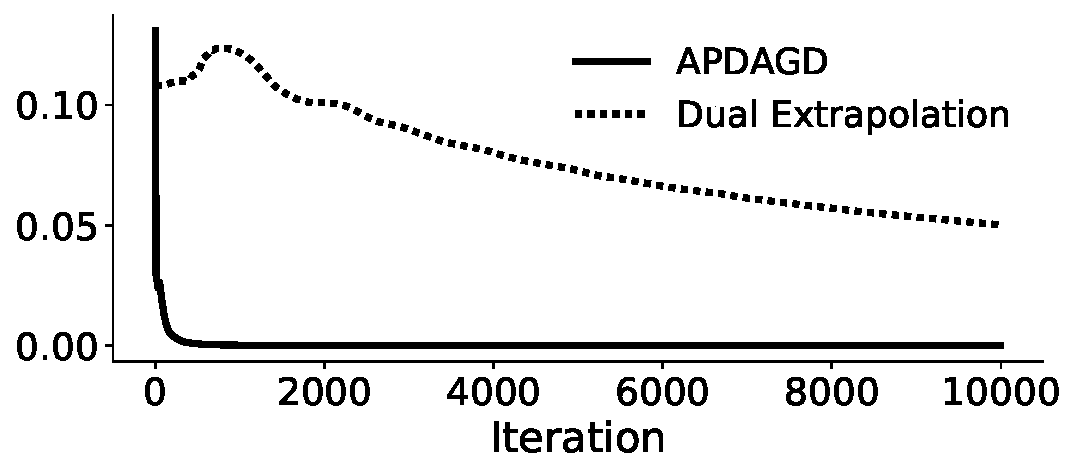
\includegraphics[width=0.45\textwidth]{figs/de_vs_apdagd_primal_gap.pdf}
    \caption{Primal optimality gap for solutions produced by APDAGD and Dual Extrapolation.}
    \label{fig:de_vs_apdagd}
\end{figure}
\begin{figure}
    \centering
    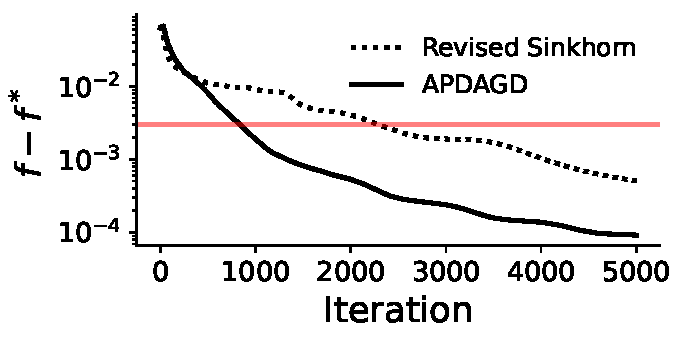
\includegraphics[width=0.9\linewidth]{figs/color_transfer_primal_opt_feasible.pdf}
    \caption{Primal optimality gap against optimization rounds achieved by our \textbf{revised} Sinkhorn and APDAGD for POT. The marginal distributions are taken from the later color transfer application in this section, and the red horizontal line depicts the pre-defined tolerance ($\varepsilon$) for both algorithms.}
    \label{fig:Feasible_Sinkhorn}
\end{figure}
\subsection{Run Time Comparison}
\textbf{APGAGD vs DE}: We are able to implement the DE algorithm for POT while the authors of DE for OT faced numerical overflow and had to use mirror prox instead “for numerical stability considerations” \cite{Jambulapati-2019-Direct}. For the setup of Figure \ref{fig:de_vs_apdagd}, we use images in the CIFAR-10 dataset \citep{krizhevsky2009learning} as the marginals. More details are included in the Further Experiment Setup Details section in Appendix. In Figure \ref{fig:de_vs_apdagd}, despite having a better theoretical complexity, DE has relatively poor practical performance compared to APDAGD. This is not surprising as previous works on this class of algorithms like \citep{pmlr-v130-dvinskikh21a} reach similar conclusions on DE's practical limitations. This can be partly explained by the large constants that are dismissed by the asymptotic computational complexity. Thus, in our applications in the following subsection, we will use APDAGD or revised Sinkhorn.

\textbf{APGAGD vs Sinkhorn}: For the same setting with CIFAR-10 dataset, we report that the ratio between the average per iteration cost of APDAGD and that of Sinkhorn is 0.68. Furthermore, in the Run Time for Varying $\varepsilon$ section in Appendix, we reproduce the same result in Figure 6 as \textbf{Figure 1 in (Dvurechensky et al., 2018)}, comparing the runtime of APDAGD and Sinkhorn for varying $\varepsilon$.


\subsection{Revised Sinkhorn}
Using the similar setting as the later example of color transfer, we can empirically verify that our revised Sinkhorn procedure can achieve the required tolerance $\varepsilon$ of the POT problem in Figure  (as opposed to pre-revised Sinkhorn in Figure \ref{fig:Infeasible_Sinkhorn}).

\subsection{Point Cloud Registration}
We now present an application of POT in point set registration, a common task in shape analysis. Start with two point clouds in three dimensions $R = \{ \vx_i \in \RR^3 \mid i = 1, \ldots, m \}$ and $Q = \{ \vy_j \in \RR^3 \mid j = 1, \ldots, n \}$. The objective is to find a transformation, consisting of a rotation and a translation, that best aligns the two point clouds. When the initial point clouds contain significant noise or missing data, the registration result is often badly aligned. Here, we consider a scenario where one set has missing values. In Figure \ref{fig:point_cloud} (a), the blue point cloud is set to contain the front half of the rabbit, retaining about 45\% of the original points. A desirable transformation must align the first halves of the two rabbits correctly.
Figure \ref{fig:point_cloud} compares the point clouds registration result using these methods. If $\vT$ is simply the OT matrix, not subject to a total transported mass constraint, the blue cloud is clearly not well-aligned with the red cloud. This is because the points for which the blue cloud is missing (i.e., the right half of the rabbit) are in the red cloud. If the total mass transported is set to $s = \frac{\min\{m, n\}}{\max\{m, n\}}$, then we end up with a POT matrix $\vT$ with all entries summing to $s$. In Figures \ref{fig:point_cloud} (c) and (d), the POT solution leads to a much better result than the OT solution: the left halves of the rabbit are closer together. Importantly, the feasible solution obtained by APDAGD leads to an even better alignment, compared to the pre-revised Sinkhorn, due to its infeasibility.

\begin{figure}
    \centering
    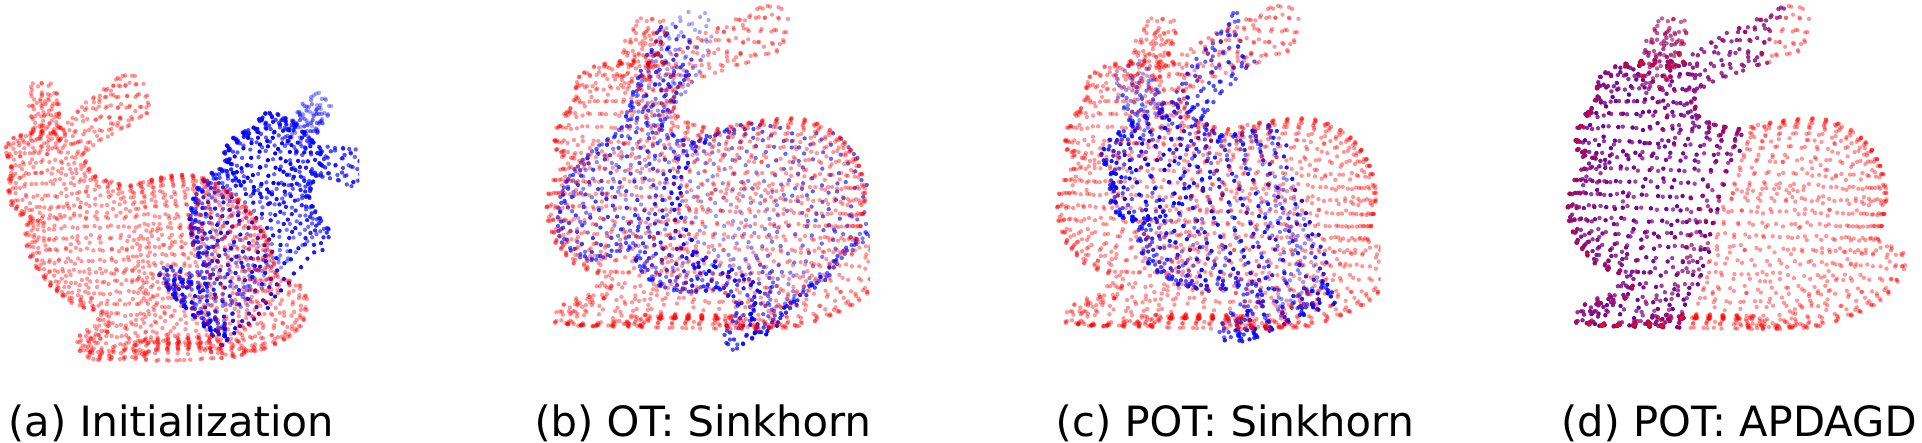
\includegraphics[width=1\linewidth]{figs/point_clouds.png}
    \caption{Point cloud registration using (partial) optimal transport. (a): Initial point sets with one set (in blue) missing 45\% of the points. (b): Registration result obtained after transforming the blue point cloud using the OT plan by Sinkhorn. (c): Registration result using the POT plan by \textbf{pre-revised} Sinkhorn \cite{nhatho-mmpot}. (d): Registration result using the POT plan by APDAGD.}
    \label{fig:point_cloud}
\end{figure}

\subsection{Color Transfer}
A frequent application of OT in computer vision is color transfer. POT offers flexibility in transferring colors between two possibly different-sized images, in contrast to OT which requires two color histograms to be normalized \citep{bonneel2015sliced}. We follow the setup by \citep{Blondel-2018-Smooth} and the detail of the implementation is described in the Further Experiment Setup Details section in Appendix. Our results are presented in Figure \ref{fig:color_transfer_comparison}. The third row of Figure \ref{fig:color_transfer_comparison} displays the resulting image produced by APDAGD with different levels of $\alpha$ (or transported mass $s$). Increasing $\alpha$ makes the wall color closer to the lighter part of the kiwi in the target image but comes at a cost of saturating the window frames' white. We emphasize that $\alpha$ is a tunable parameter, and the user can pick the most suitable level of transported mass. This can be more flexible than the vanilla OT which stringently requires all marginal masses to be normalized. We also emphasize that qualitatively, the solution produced by APDAGD closely matches the exact solution in (d), in contrast to \textbf{pre-revised} Sinkhorn's \cite{nhatho-mmpot}. This highlights the impact of having a feasible and optimal mapping on the quality of the application. 

\begin{figure}
    \centering
  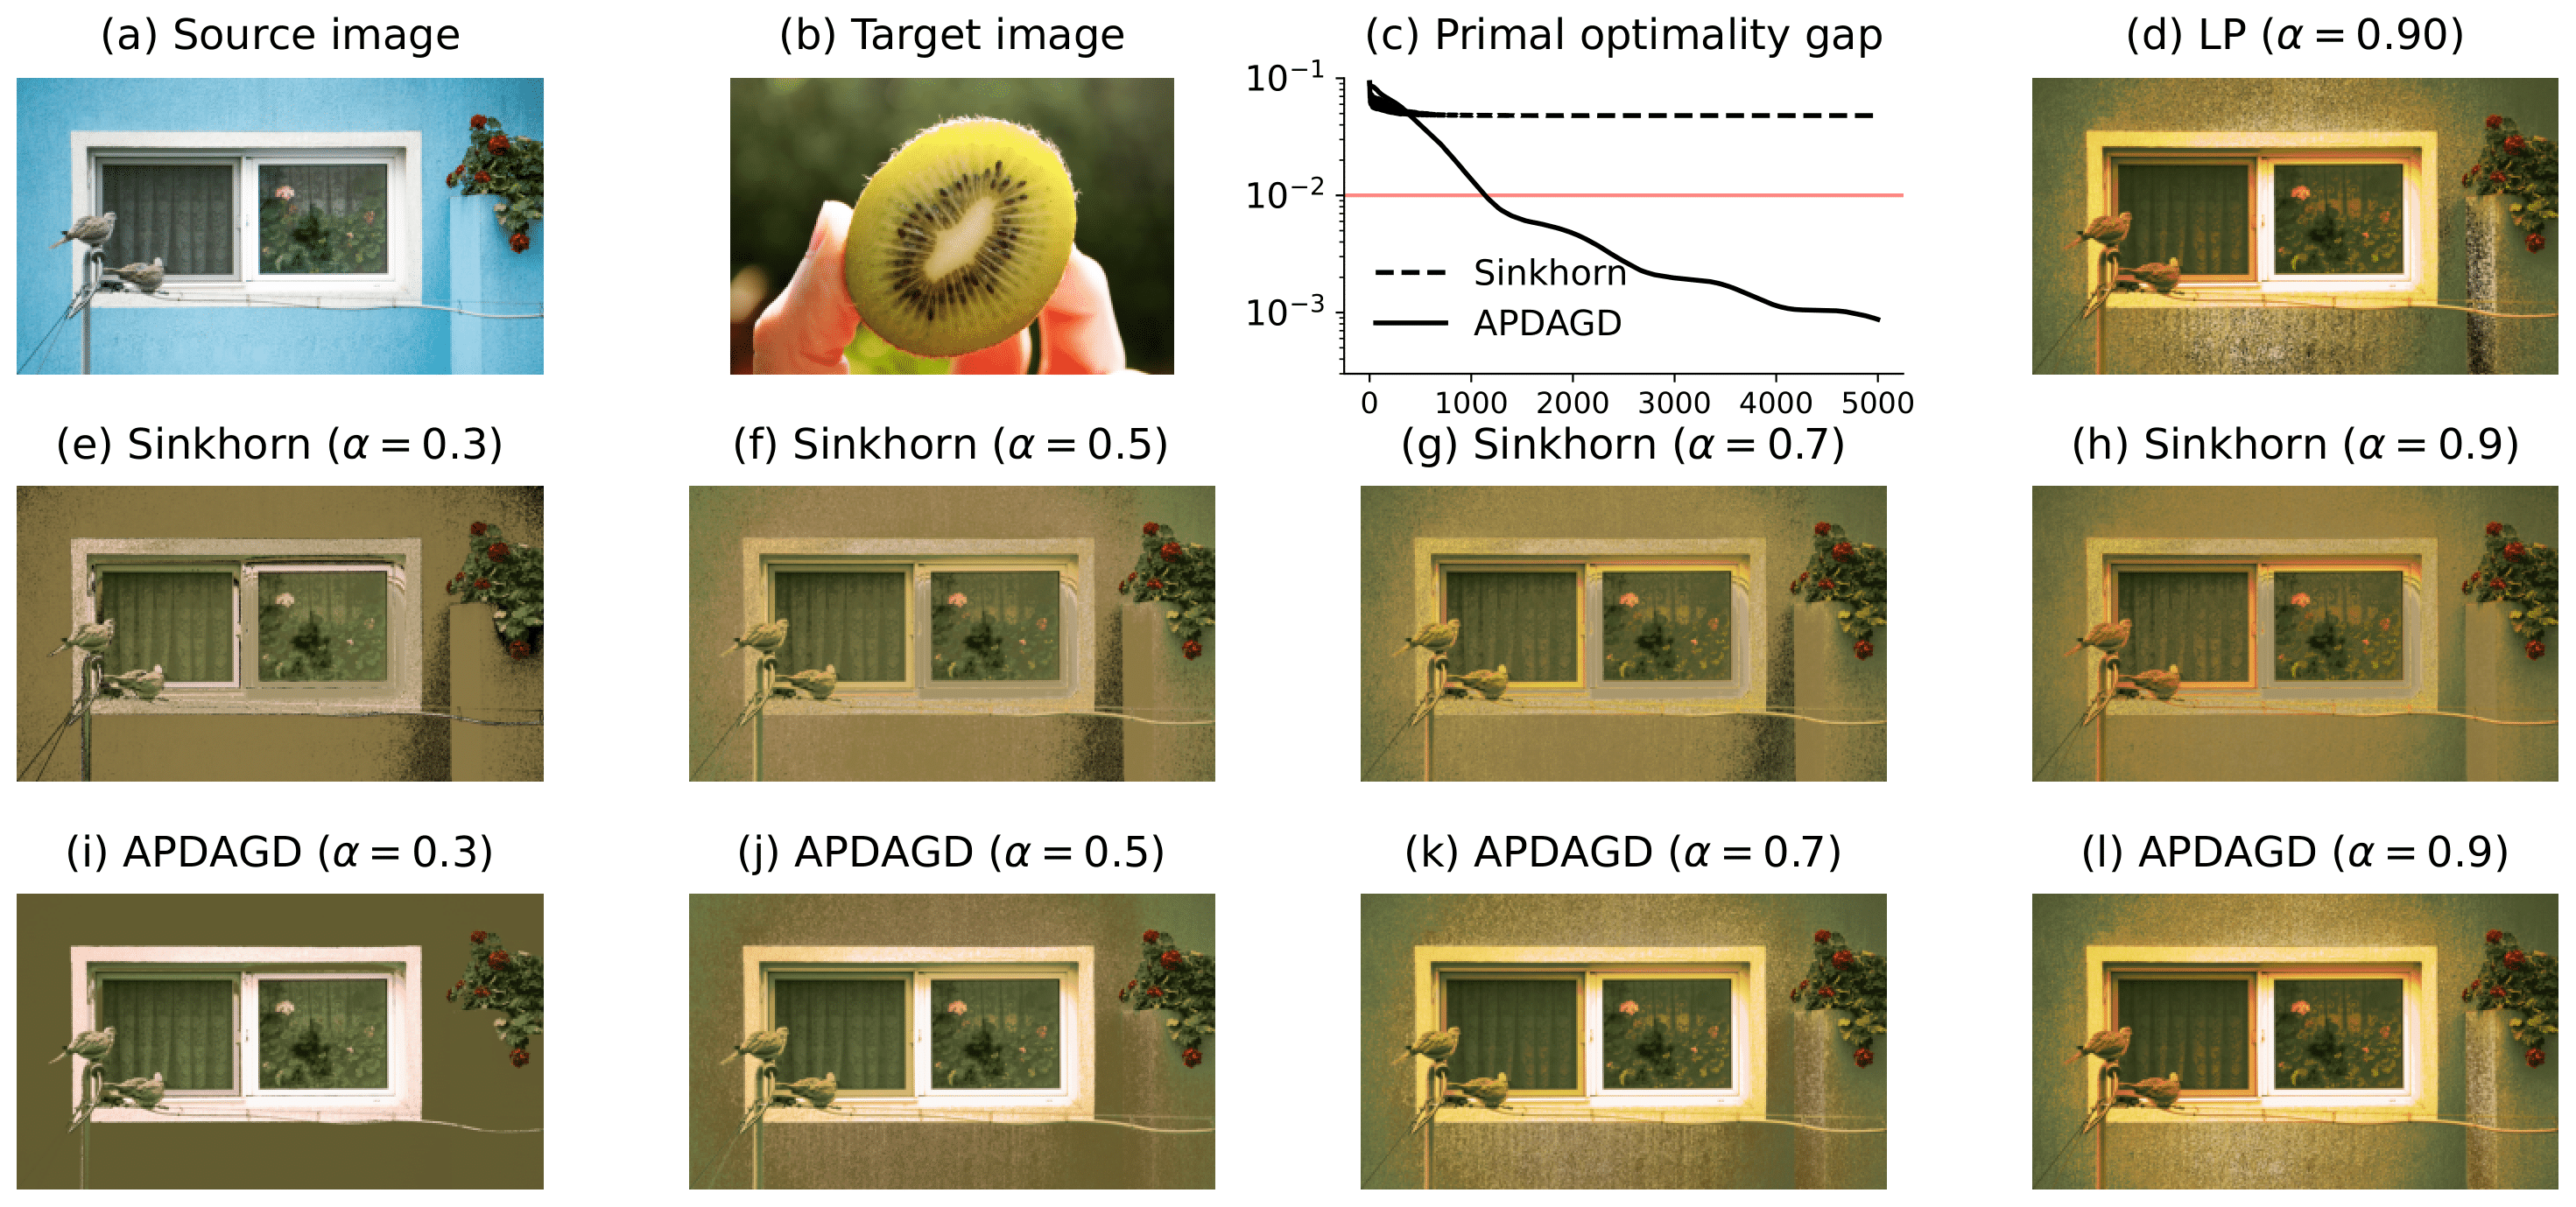
\includegraphics[width=1\linewidth]{figs/color_transfer_all.png}
  \caption{Color transfer using POT. The source and target images are of different sizes, giving rise to unbalanced color histograms. We apply Sinkhorn and APDAGD to solve the entropic regularized POT problem between these histograms. The optimality gap $\inner{\vC}{\vX} - f^*$ after each iteration is displayed in (c). The exact solution, retrieved by the Gurobi solver is presented in (d). On the second and third rows, the transformed image is displayed for different levels of $\alpha$, showing the flexibility of POT as opposed to OT.}  
  \label{fig:color_transfer_comparison}
\end{figure}